%%
%% This is file `sample-sigconf.tex',
%% generated with the docstrip utility.
%%
%% The original source files were:
%%
%% samples.dtx  (with options: `sigconf')
%% 
%% IMPORTANT NOTICE:
%% 
%% For the copyright see the source file.
%% 
%% Any modified versions of this file must be renamed
%% with new filenames distinct from sample-sigconf.tex.
%% 
%% For distribution of the original source see the terms
%% for copying and modification in the file samples.dtx.
%% 
%% This generated file may be distributed as long as the
%% original source files, as listed above, are part of the
%% same distribution. (The sources need not necessarily be
%% in the same archive or directory.)
%%
%% The first command in your LaTeX source must be the \documentclass command.
\documentclass[sigconf]{acmart}

\usepackage{amsmath,amssymb}
\usepackage{amsfonts}
\usepackage{subfigure}
\usepackage{multirow}
\usepackage{IEEEtrantools}

%%
%% \BibTeX command to typeset BibTeX logo in the docs
\AtBeginDocument{%
  \providecommand\BibTeX{{%
    \normalfont B\kern-0.5em{\scshape i\kern-0.25em b}\kern-0.8em\TeX}}}

%% Rights management information.  This information is sent to you
%% when you complete the rights form.  These commands have SAMPLE
%% values in them; it is your responsibility as an author to replace
%% the commands and values with those provided to you when you
%% complete the rights form.
\copyrightyear{2019}
\acmYear{2019}
\setcopyright{rightsretained}

%% These commands are for a PROCEEDINGS abstract or paper.
%\acmConference{SIGGRAPH '19 Talks}{July 28 - August 01, 2019}{Los Angeles, CA, USA}
%\acmDOI{10.1145/3306307.3328180}
%\acmISBN{978-1-4503-6317-4/19/07}
%\acmBooktitle{SIGGRAPH '19 Talks, 
%  July 28 - August 01, 2019, Los Angeles, CA}


%%
%% Submission ID.
%% Use this when submitting an article to a sponsored event. You'll
%% receive a unique submission ID from the organizers
%% of the event, and this ID should be used as the parameter to this command.
%%\acmSubmissionID{123-A56-BU3}

%%
%% The majority of ACM publications use numbered citations and
%% references.  The command \citestyle{authoryear} switches to the
%% "author year" style.
%%
%% If you are preparing content for an event
%% sponsored by ACM SIGGRAPH, you must use the "author year" style of
%% citations and references.
%% Uncommenting
%% the next command will enable that style.
%%\citestyle{acmauthoryear}

%%
%% end of the preamble, start of the body of the document source.
\begin{document}

%%
%% The "title" command has an optional parameter,
%% allowing the author to define a "short title" to be used in page headers.
\title{Wi-Fi Based Handwritten Signature Verification Using a Triplet Network}

%%
%% The "author" command and its associated commands are used to define
%% the authors and their affiliations.
%% Of note is the shared affiliation of the first two authors, and the
%% "authornote" and "authornotemark" commands
%% used to denote shared contribution to the research.
\author{Young-Woong Kwon, Jooyoung Kim and Kar-Ann Toh}
%\authornote{Both authors contributed equally to this research.}
\affiliation{%
  \institution{School of Electrical and Electronic Engineering, Yonsei University}
  \streetaddress{50 Yonsei-ro}
  \city{Seodaemun-gu}
  \state{Seoul}
  \country{Korea}
  \postcode{03722}
}
%\email{herokwon@yonsei.ac.kr}

%%
%% By default, the full list of authors will be used in the page
%% headers. Often, this list is too long, and will overlap
%% other information printed in the page headers. This command allows
%% the author to define a more concise list
%% of authors' names for this purpose.
\renewcommand{\shortauthors}{Y.Kwon, et al.}

%%
%% The abstract is a short summary of the work to be presented in the
%% article.
\begin{abstract}
    In this paper, we propose a system for identity verification based on the handwritten signature signals captured by the Wi-Fi Channel State Information (CSI). 
    To facilitate a fast converging loss model, a kernel and the range space learning is initially adopted for mining the triplet inputs. 
    Subsequently, the triplet network is trained on a ConvNet structure using the mined triplet inputs. 
    Our experiments on an in-house Wi-Fi handwritten signature signal dataset show encouraging verification accuracy with faster training loss convergence comparing with the baseline triplet network and the Siamese network.
\end{abstract}

%%
%% The code below is generated by the tool at http://dl.acm.org/ccs.cfm.
%% Please copy and paste the code instead of the example below.
%%

\begin{CCSXML}
    <ccs2012>
    <concept>
    <concept_id>10002978.10002991.10002992.10003479</concept_id>
    <concept_desc>Security and privacy~Biometrics</concept_desc>
    <concept_significance>500</concept_significance>
    </concept>
    <concept>   
    <concept_id>10010147.10010257.10010293.10010294</concept_id>
    <concept_desc>Computing methodologies~Neural networks</concept_desc>
    <concept_significance>500</concept_significance>
    </concept>
    </ccs2012>
\end{CCSXML}
    
\ccsdesc[500]{Security and privacy~Biometrics}
\ccsdesc[500]{Computing methodologies~Neural networks}

%%
%% Keywords. The author(s) should pick words that accurately describe
%% the work being presented. Separate the keywords with commas.
\keywords{Wi-Fi signature signal, in-air handwritten signature verification, the Kernel and the Range space projection learning, triplet network.}

%% A "teaser" image appears between the author and affiliation
%% information and the body of the document, and typically spans the
%% page.
%\begin{teaserfigure}
%  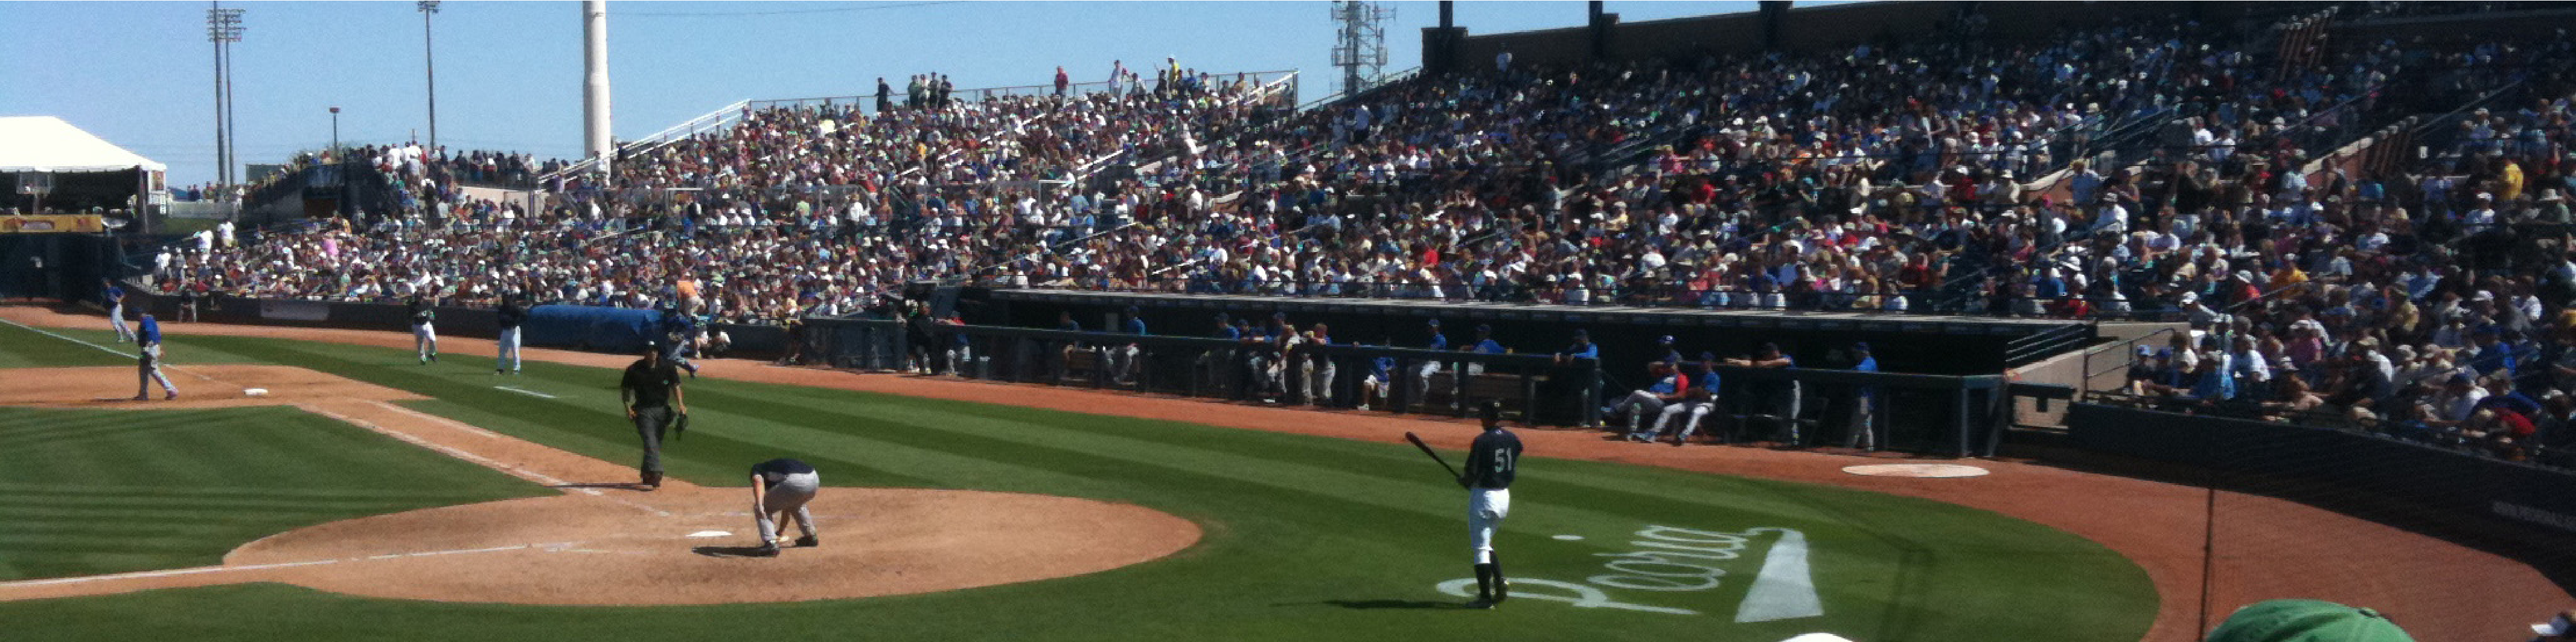
\includegraphics[width=\textwidth]{sampleteaser}
%  \caption{Seattle Mariners at Spring Training, 2010.}
%  \Description{Enjoying the baseball game from the third-base
%  seats. Ichiro Suzuki preparing to bat.}
%  \label{fig:teaser}
%\end{teaserfigure}

%%
%% This command processes the author and affiliation and title
%% information and builds the first part of the formatted document.
\maketitle

%Intro
\section{Introduction}
Over recent years, several behavioral biometric traits attracted attention in view of their rigid physical body independence~\cite{bailador2011analysis}. Among these behavioral biometrics, the signature-based user authentication~\cite{fahmy2010online,sanmorino2012survey,galbally2015line} has attracted considerable interest with the development of in-air signature recognition systems~\cite{jeon2012system,malik20183dairsig,ketabdar2012magnetic}.
With the help of sensors such as the depth camera~\cite{jeon2012system,malik20183dairsig} or a mobile sensor~\cite{ketabdar2012magnetic}, the in-air signature recognition system has lower the spatial constraint in the process of signature acquisition comparing with contact-based authentication systems~\cite{jeon2012system,malik20183dairsig,ketabdar2012magnetic,sesa2012information}.

Recently, the commercial Wi-Fi device has been adopted for in-air signature authentication due to its easy accessible property \cite{moon2017air}. Based on the distortion of the  Wi-Fi CSI signal according to the user's gestures, the in-air signature recognition system showed reasonable user verification performance~\cite{moon2017air}. More recently, some studies attempted to implement the deep learning algorithms in Wi-Fi signal-based user authentication systems to improve the verification performance ~\cite{shi2017smart,pokkunuru2018neuralwave}. 

In this paper, we utilize a deep triplet network for identity verification based on the Wi-Fi CSI signature signal. To achieve not only the desired verification accuracy but also a fast training speed, we adopt the kernel and the range (KAR) space learning~\cite{toh100,toh2018learning,toh2018analytic,toh2018gradient} in order to mine the distinctive triplet inputs. Subsequently, the triplet network which utilizes the ConvNet structure as a feature extractor is trained based on the $L2$ distance comparison.

The main contributions of our work can be summarized as follows:
\begin{itemize}
\item Proposal of a system for identity verification based on the Wi-Fi handwritten signature signals using a deep triplet network.
\item Adopted the kernel and the range (KAR) space learning in order to mine the distinctive triplet inputs which boost the convergence speed of the training loss in the triplet network.
\item Provision of an experimental study using an in-house Wi-Fi handwritten signature dataset collected from 50 subjects.
\end{itemize}

The paper is organized as follows: related works including the triplet network and KAR space learning are introduced in Section 2 for immediate reference. Our proposed method is discussed in Section 3. Section 4 describes our experimental results and analysis. Some concluding remarks are given in Section 5.

\section{Related works}

\subsection{Triplet network}
% triplet network
The triplet network is considered a metric learning based model~\cite{weinberger2006distance} which aims to learn useful representations by means of distance comparison~\cite{hoffer2015deep}. 
It is often seen in person re-identification~\cite{chen2017beyond,cheng2016person,ding2015deep,schroff2015facenet,wang2016joint} where the individual identities are matched based on discriminative image features. The main difference between person identification and re-identification is that the later is a more challenging task where images of the same person taken from different cameras or under different occasions are to be associated. In order to address our challenging Wi-Fi based verification task, we adopt a triplet network which optimizes the input data space so that data points with the same identity are closer to each other than those with different identities~\cite{hermans2017defense}.

The triplet network receives triplet pairs of data as its input. These data triplets are constructed based on a combination of the input data. Since not all triplet samples contribute to the desired classification, recent attention~\cite{schroff2015facenet} has been paid to the choice of relevant input pairs for training. In order to optimize the training process which utilizes only some parts of the triplet pairs, several researches~\cite{cheng2016person,ding2015deep,wang2016joint} generated triplets from a small number of classes (persons) in each iteration. Recently, \cite{schroff2015facenet} adopted a triplet mining process to speed up the training convergence. They utilized a large mini-batch at each training iteration and selected the triplets based on network training instead of random sampling. However, this strategy needed a few thousands of exemplar mini-batches in every training iteration for triplet pairs selection. This results in a heavy computational load in training. In order to make use of the small sample training size as well as to speed up the triplet training process, we adopt the kernel and range space method for the learning.

% Rel works: KAR learning
\subsection{Kernel and the range space learning}\label{kar}

Generally, the multilayer feedforward neural networks is trained based on the gradient descent method via backpropagation~\cite{goodfellow2016deep}.
However, setting the learning parameters such as the learning rate and the learning momentum is a time consuming task.

Recently, a gradient-free learning framework based on the kernel and the range (KAR) space manipulation has been developed for multilayer network learning~\cite{toh100,toh2018learning,toh2018analytic,toh2018gradient}.
The learning method is grounded on linear algebra with neither learning parameters nor iteration is needed in training.

% Karnet structure and mining samples.
Given $m$ training samples. Let $\mathbf{X}\in{\mathbb{R}}^{m \times (n+1)}$ denotes the training data set and $\mathbf{G}\in{\mathbb{R}}^{m \times n}$ denotes the network output.
Then the multilayer neural network can be written in equation form as follows:
\begin{IEEEeqnarray}{rCl}
    \mathbf{G}&=&\sigma\left(\left[\mathbf{1},\sigma\left(\dots\left[\mathbf{1},\sigma\left(\left[\mathbf{1},\sigma\left(\mathbf{X}\mathbf{W}_{1}\right)\right]\mathbf{W}_{2}\right)\right]\dots\mathbf{W}_{(i-1)}\right)\right]\mathbf{W}_{i}\right), \nonumber \\ i&=&1,\dotsc,n,
\end{IEEEeqnarray}
where $\mathbf{W}_{1}\in{\mathbb{R}}^{(n+1) \times h_{1}}$,$\mathbf{W}_{2}\in{\mathbb{R}}^{(h_{1}+1) \times h_{2}}$,$\dots,\mathbf{W}_{i}\in{\mathbb{R}}^{(h_{(i-1)}+1) \times n}$ are the network weight matrices, $\mathbf{1}=\left[1,\dots,1\right]^{T}\in{\mathbb{R}}^{m \times 1}$ is the bias vector, and $\sigma(.)$ is the activation function.
By adopting an one-hot encoded target $\mathbf{Y}\in{\mathbb{R}}^{m \times n}$, training of the weight matrices $\mathbf{W}_{i}$ using the KAR space method~\cite{toh2018gradient} can be computed as follows:
\begin{IEEEeqnarray}{rCl}
    \mathbf{W}_{i}&=&\left[\mathbf{1},\sigma\left(\dots\left[\mathbf{1},\sigma\left(\left[\mathbf{1},\sigma\left(\mathbf{X}\mathbf{W}_{1}\right)\right]\mathbf{W}_{2}\right)\right]\dots\mathbf{W}_{(i-1)}\right)\right]^{\dagger}\sigma^{-1}\left(\mathbf{Y}\right), \nonumber \\ i&=&1,\dotsc,n.
\end{IEEEeqnarray}

%% Methods
\section{Proposed System}

% Methods: System overview(Fig.1)
In this section, we propose an identity verification system based on the Wi-Fi in-air handwritten signature (which will be called Wi-Fi signature hereafter) using the triplet network~\cite{hoffer2015deep}. Fig.1 shows an overview of the proposed system utilizing the kernel and the range (KAR) space learning~\cite{toh2018learning,toh2018gradient} for mining the triplet inputs.
Essentially, the KAR space projection learning is utilized to learn the triplet input data by mining the hard positive and the hard negative samples from each of the given anchor sample (see item (a) in Fig.~\ref{fig1}). The hard positive and the hard negative samples refer to positive and negative class samples which are likely to be misclassified by the network.
Subsequently, the ConvNet structure in the triplet network (see item (b) in Fig.~\ref{fig1}) is trained with the mined triplet data based on a triplet loss function using the $L2$ distance comparison (see item (c) in Fig.~\ref{fig1}).
The following subsections describe the details of the triplet mining using KAR space learning and the triplet network.

% Figure 1
\begin{figure*}[!ht]
    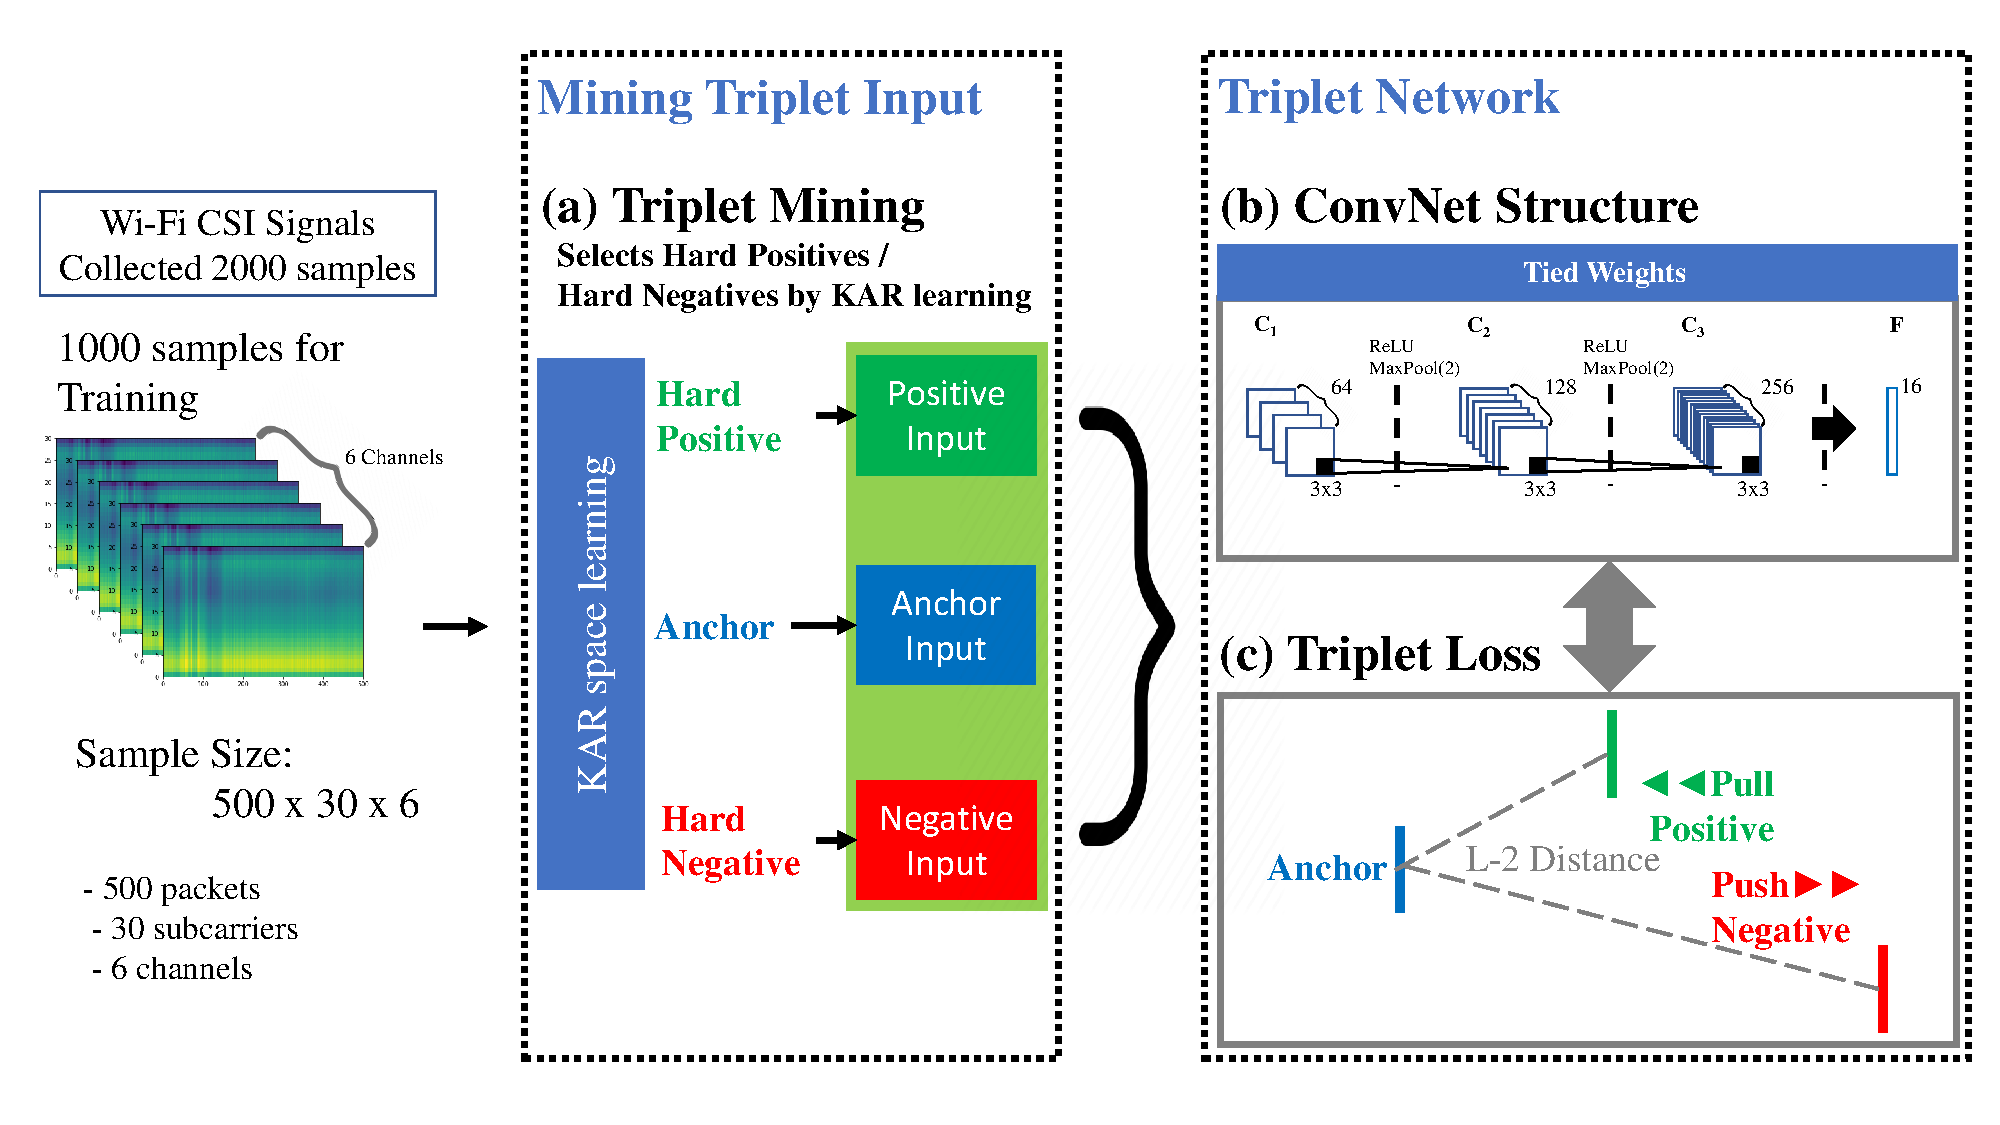
\includegraphics[width=\textwidth]{fig1_tcnn_kar_v6}
    \caption{An overview of the proposed system.} \label{fig1}
\end{figure*}

% Methods: KAR learning
\subsection{Triplet mining using the kernel and the range space learning}

The network receives a triplet set of data as its inputs. These triplet data consist of the reference data (will be called anchor samples hereafter) and the corresponding positive class data (same class with that of the anchor) and the negative class data (different class from that of the anchor). The goal of the triplet network is to position the feature vectors with appropriate separation space by putting the positive samples close to the anchor sample while keeping the negative sample away from the anchor sample.

According to \cite{schroff2015facenet}, it is important to select the hard positive samples and the hard negative samples with reference to the given anchor sample for fast loss convergence when training the triplet network.
A hard positive sample is defined as a sample whose distance to the anchor sample is large (which is most likely to be misclassified as a negative sample). On the other hand, a hard negative sample is defined as a sample whose distance to the anchor sample is small (which is most likely to be misclassified as a positive sample). However, from the raw data, there is no information regarding whether a sample is considered hard positive or hard negative before we train the network.

In this work, we propose to adopt the kernel and the range (KAR) space learning (see Section~\ref{kar} for details) as a pretraining network to mine the hard positive/negative samples from the given anchor sample. Since the KAR space learning has no iterative learning process, we can mine the triplet samples without using the time consuming backpropagation training process.
 
By training the network with the single shot KAR space learning, we can map the $L2$ distance between every sample by using the output vector of the KAR space network. Given a set of training data which is packed in matrix $\mathbf{X}$, the network output can be written as:
\begin{IEEEeqnarray}{rCl}
    f\left(\mathbf{X}\right) &=& \sigma\left(\left[\mathbf{1},\sigma\left(\dots\left[\mathbf{1},\sigma\left(\left[\mathbf{1},\sigma\left(\mathbf{X}\cdot\mathbf{W}_{1}\right)\right]\mathbf{W}_{2}\right)\right]\dots\mathbf{W}_{(i-1)}\right)\right]\mathbf{W}_{i}\right), \nonumber \\ i&=&1,\dotsc,n.
\end{IEEEeqnarray}
After training based on the KAR space projection, the given anchor sample $\mathbf{x}_{anc}$ can be used as the reference to decide whether the network output of a sample is far away from this anchor sample. In other words, a hard positive sample $\mathbf{x}_{pos}$ and a hard negative sample $\mathbf{x}_{neg}$ with respect to the anchor sample $\mathbf{x}_{anc}$ can each be determined based on:
\begin{equation}
    {\left\| {{f\left(\mathbf{x}_{anc}\right)} - {f\left(\mathbf{x}_{pos}\right)}} \right\|_2^2} \geq \mathrm{t}_{pos}, \label{pos}
\end{equation}
\begin{equation}
    {\left\| {{f\left(\mathbf{x}_{anc}\right)} - {f\left(\mathbf{x}_{neg}\right)}} \right\|_2^2} \leq \mathrm{t}_{neg},\label{neg}
\end{equation}
where $\mathrm{t}_{pos}$ and $\mathrm{t}_{neg}$ respectively denote the thresholds that determine whether a sample is hard positive or hard negative. Since the hardest samples are likely to be outliers which can degrade the training process of the triplet network, we empirically set the $\mathrm{t}_{pos}$ at 75 percentile of the $L2$ distance and $\mathrm{t}_{neg}$ at 25 percentile of the $L2$ distance. The final set of $\mathbf{x}_{pos}$ and $\mathbf{x}_{neg}$ samples is randomly selected based on equations~\eqref{pos} and~\eqref{neg}.

% Methods: ConvNets
\subsection{The ConvNet structure}

The next step is to design a feature extractor which converts the  triplet input data into feature vectors. In this work, we utilize the ConvNet structure~\cite{lecun1998gradient} as a feature extractor since the three dimensional data format of our preprocessed input signal can be regarded as an image data format with multiple channels. 

Our ConvNet design (item (b) in Fig~\ref{fig1}) consists of three convolutional layers and one fully-connected layer. The number of convolutional filters to be trained in each layer is empirically chosen as $\{64, 128, 256\}$, with fixed filter size of $3\times3$, each of stride 1. The Rectified Linear (ReLU) activation function and the Max-pooling layer are applied between each convolutional layer. Subsequently, the extracted features from the last convolutional layer are flattened into a vector before feeding into the fully-connected network.
The output vectors from the fully-connected layer are finally transformed using the sigmoid function followed by a $L2$ normalization.

% Methods: Triplet loss
\subsection{The triplet loss}

The triplet loss function was first seen in \cite{hoffer2015deep} for training the triplet network. For the $i^{th}$ network input $\left\{\mathbf{x}_{anc,i}, \mathbf{x}_{pos,i}, \mathbf{x}_{neg,i}\right\}$, an anchor sample $\mathbf{x}_{anc,i}$ is randomly selected among the training data set. The positive and negative samples (respectively $x_{pos,i}$ and $x_{neg,i}$) are then determined and being selected for training the ConvNet based on the feature vectors $\left\{\mathbf{v}_{anc,i},\mathbf{v}_{pos,i},\mathbf{v}_{neg,i}\right\}$, for i=1,...,N.
The triplet loss function is formulated based on a summation of the difference between the positive distance (the $L2$ distance between the anchor vector and the positive vector) and the negative distance (the $L2$ distance between the anchor vector and the negative vector) as follows:
\begin{equation}
    loss = \sum_i^N max\left({ \left[ {\left\| {{\mathbf{v}_{anc,i}} - {\mathbf{v}_{pos,i}}} \right\|_2^2} - {\left\| {{\mathbf{v}_{anc,i}} - {\mathbf{v}_{neg,i}}} \right\|_2^2}  + \alpha \right]},0 \right),\label{triplet}
\end{equation}
where $N$ denotes the size of the mini-batch, ${\left\| . \right\|_2^2}$ denotes the $L2$ distance and $\alpha$ denotes the preset margin.
The ConvNet structure using equation~\eqref{triplet} is trained to maximize the gap between the positive distance and the negative distance which should be larger than the margin $\alpha$.

\section{Experiments}

% Dataset
\subsection{Dataset}
 In order to evaluate the verification performance of the proposed system, the Wi-Fi CSI signature dataset \cite{moon2017air} is utilized in our experiments. The Wi-Fi CSI signature dataset consists of 2000 Wi-Fi CSI signature signals (4 directions $\times$ 10 samples $\times$ 50 identities) with sample size 500$\times$30$\times$6. We utilize only the absolute value from each complex CSI signal in our experiments.

\subsection{Experimental settings}

\subsubsection{Performance evaluation:}
The proposed system is evaluated under two cases: i) case I on comparison between the proposed system and other handcraft or deep learning-based methods based on the verification accuracy, and case II on detailed comparison between the proposed system and the deep learning-based methods using the receiver operating characteristic (ROC) curve and training loss curve. For both cases, Wi-Fi signal measurements based on a single-orientation and 4-orientations of the user are recorded. For Case I, existing handcraft methods such as the least squares error estimation (LSE)~\cite{duda2012pattern}, the principal components analysis (PCA) [22] with LSE, the support vector machine (SVM)~\cite{vapnik2013nature} with different kernel functions, the total error rate minimization which adopted the reduced multivariate polynomial model as basis function (TER-RM2) \cite{toh2003fingerprint,toh2008between}, the deep learning-based Siamese network \cite{koch2015siamese}, and the baseline triplet network \cite{hoffer2015deep} are included for performance benchmarking. The Siamese network and the baseline triplet network utilized the same ConvNet structures with the proposed system and only differed in their input data style and loss function.

The verification performance of the proposed system and the compared methods are evaluated in terms of the Equal Error Rate (EER, \%) which are taken from averaging the results of five runs of two-fold cross-validation tests. Due to the memory constraint caused by the large data size, the deep learning-based methods utilized randomly sampled 9,500 negative pairs in the validation stage, which is the same number as the number of positive pairs.

\subsubsection{Network Structure and Parameter Settings:}
The multilayer feedforward network structure of KAR space learning is specified in Table~\ref{tab2}. With input data, size of 500$\times$30$\times$6, we set two network layers where the size of the each layer is 1024 and 16, respectively. Each layer is initialized with uniform distribution over [0, 1). We used $\sigma = {tan}^{-1}$ as the activation function following \cite{toh2018analytic}.
\begin{table}
    \caption{The network structure of KAR space learning.}
    \label{tab2}
    \begin{tabular}{ccc}
     \toprule
     Layer   & Size     & Activation \\
     \midrule
     Input   & 500$\times$30$\times$6 &            \\
     Fully-Connected 1 & 1$\times$1$\times$1024 & $\sigma = {tan}^{-1}$     \\
     Fully-Connected 2 & 1$\times$1$\times$16  & $\sigma = {tan}^{-1}$     \\
     Output  & 1$\times$1$\times$50   &            \\
     \bottomrule
    \end{tabular}
\end{table}

For the proposed system and the deep learning-based methods, we utilized the same ConvNet structure as specified in Table~\ref{tab1}. We trained the network starting with a learning rate of 0.00005 and a mini-batch size of 32. We optimized the loss by the Adam optimizer with $L2$ penalty of 0.0002 except for the output layer. The output layer was regularized using an $L2$ penalty of 0.0001. We initialized all network weights in the convolutional layers with normal distribution of zero-mean and standard deviation 0.01. The biases were also initialized with a normal distribution of 0.5 mean and standard deviation 0.01. For the triplet networks, the hyper-parameter regulating triplet loss is empirically set at 0.1. The training epochs were set at 1,500 for all three deep learning-based algorithms. For the linear methods such as LSE, SVM and TER, the input signals were resized to 500 $\times$ 30 by averaging along the subcarrier axes due to limitation of hardware memory. For the PCA-LSE, the input dimension was reduced to 40.
\begin{table}
    \caption{The structure of ConvNet model. For the convolution layer, the kernel is specified as (m$\times$m) sized filter $\times$ (\# of filters) / (\# of stride). For the max-pooling layer, (p$\times$p) sized pooling windows / \# of stride. The input sizes are denoted as rows $\times$ cols $\times$ \# of filters.}
    \label{tab1}
    \begin{tabular}{cccc}
     \toprule
     Layer     & Activation & Kernel / Stride & Input Size \\
     \midrule
     Conv 1    & ReLU       & (3$\times$3)$\times$64/1      & 500$\times$30$\times$6   \\
     MaxPool 1 &            & (2$\times$2)/1         & 500$\times$30$\times$64  \\
     Conv 2    & ReLU       & (3$\times$3)$\times$128/1     & 250$\times$15$\times$64 \\
     MaxPool 2 &            & (2$\times$2)/1         & 250$\times$15$\times$128 \\
     Conv 3    & ReLU       & (3$\times$3)$\times$256/1     & 125$\times$8$\times$128  \\
     MaxPool 3 &            & (2$\times$2)/1         & 125$\times$8$\times$256  \\
     Fully-Connected     & Sigmoid    & 16             & 63$\times$4$\times$256   \\
     $L2$ Norm  &            &                 & 1$\times$1$\times$16    \\
     Concat    &            &                 & 1$\times$1$\times$16    \\
     \bottomrule
    \end{tabular}
\end{table}

\subsection{Results and discussion}

Case I: Table~\ref{tab3} shows the average of EER performance from five runs of two-fold cross-validation tests under the optimal parameter setting. For 1-orientation inputs, SVM showed the best verification accuracy of 1.55\% EER. However, For 4-orientation inputs, all three deep learning-based methods showed better performance than hand-craft methods. This is, perhaps, due to the utilization of the original size (500$\times$30$\times$6) of the input data in the training stage for the deep learning based methods. The test EER performance of the proposed system is 19.35\%. The baseline triplet network without input mining showed slightly worse performance of 20.34\% EER. The Siamese network showed the worst verification performance of 23.53\% EER. The Siamese network is also a metric learning system, but differs from our system in that it receives two inputs and uses the contrastive loss function for training. 
\begin{table*}
    \caption{Performance benchmarking with respect to the best EER (\%) averaged from five runs of two-fold cross-validation tests.}
    \label{tab3}
    \begin{tabular}{cccl}
    \toprule
    \multirow{2}{*}{Methology} & \multicolumn{2}{c}{Best EER (\%)} & \multirow{2}{*}{Parameter setting} \\ \cline{2-3}           & 1-orientation & 4-orientation     &    \\
    \midrule
    LSE                                    & 35.40 & 48.44           &                           \\ 
    PCA-LSE                                & 16.87 & 30.79           & Reduced dimension=40        \\ 
    SVM(Linear)                            & 1.55 & 28.23            & c=1                        \\ 
    SVM(RBF)                               & 3.97 & 24.31            & c=1, $\gamma$=0.01/3000    \\ 
    TER-RM2                                & 13.29 & 35.84          & M=1,$\tau$=$\eta$=0.5      \\
    \midrule
    Siamese network                        & 16.86 & 23.53           & lr=0.00005                 \\ 
    Baseline triplet network               & 5.45 & 20.34           & lr=0.00005, $\alpha$=0.1   \\ 
    \textbf{Proposed system}               & \textbf{5.09} & \textbf{19.35}           & \textbf{lr=0.00005, $\alpha$=0.1}   \\
    \bottomrule
    \end{tabular}
\end{table*}

Case II: Fig.~\ref{fig2} (a) shows the ROC curves of the three compared deep learning-based methods. As shown in the figure, the proposed system clearly shows the largest Area Under Curve (AUC) among three compared methods. In Fig.\ref{fig2} (b) the training loss trends are plotted with respect to along the number of training iterations. Here, the proposed system shows the fastest training loss convergence followed by the baseline triplet network. In the figure, the y-axes of triplet network based methods and the Siamese network are normalized into $[0,1]$ since each loss function has different starting value. According to these observations, it can be concluded that the triplet input mining with KAR space learning improves not only the verification performance but also the training loss convergence speed.
% Figure 2,3
\begin{figure}[!ht]
    \begin{center}
    \subfigure[][ROC Curve]{
        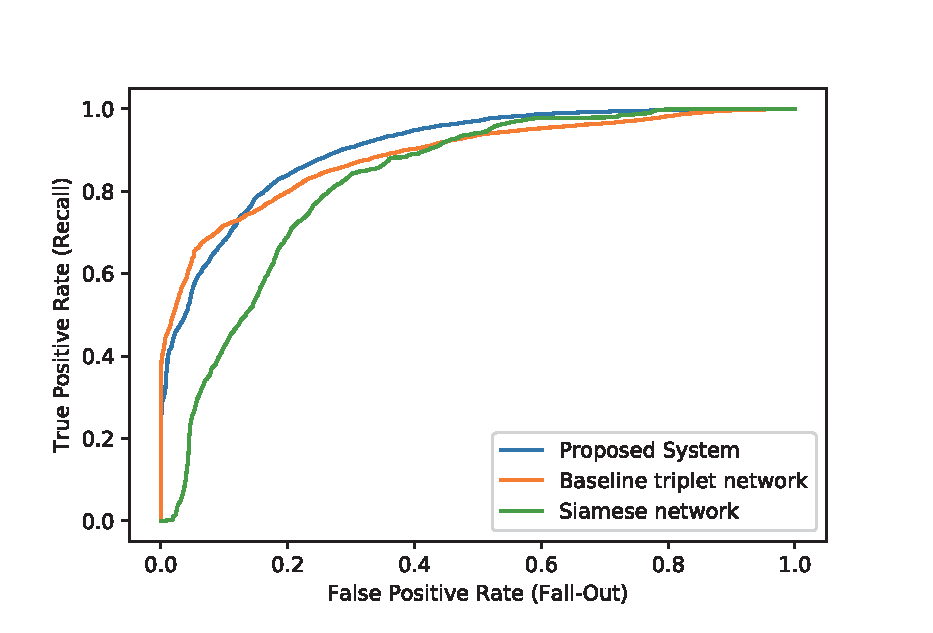
\includegraphics[height=6.4cm]{fig_roc_v14.eps}}
    \subfigure[][Normalized training loss curve]{
        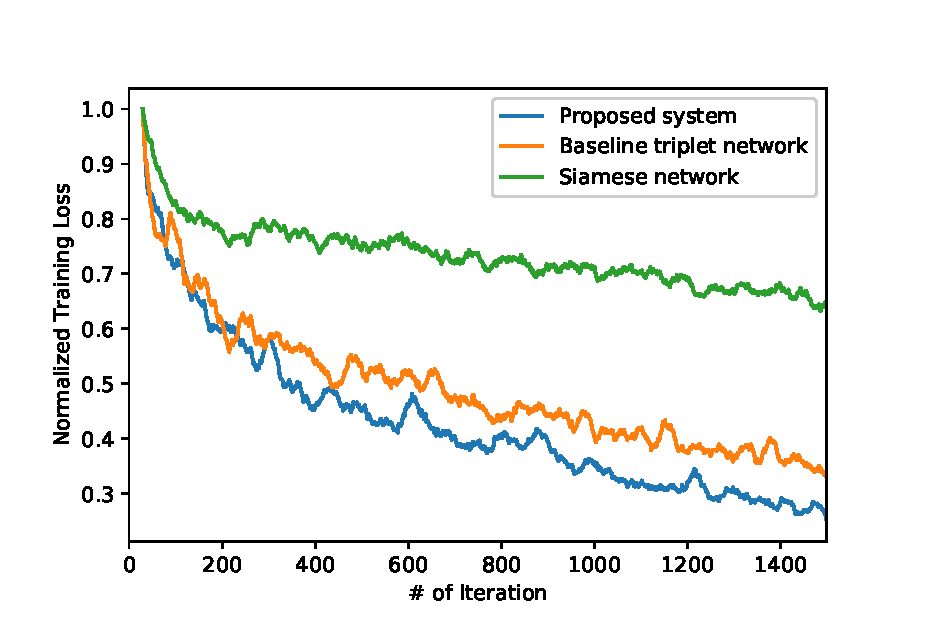
\includegraphics[height=6.4cm]{normalized_loss_curve_ma30_v2.eps}}
    \caption{(a) Receiver Operating Characteristic (ROC) Curves and 
    (b) normalized training loss trends}
    \label{fig2}
    \end{center}
 \end{figure}

\section{Conclusion}
In this paper, we proposed a system for identity verification based on the handwritten signature signals captured by the Wi-Fi Channel State Information (CSI). 
The kernel and the range space learning was adopted for mining the triplet inputs for fast loss convergence. 
Subsequently, the triplet network utilizing the ConvNet structure was trained with the mined triplet inputs based on the $L2$ distance comparison. 
Our experiments on an in-house Wi-Fi handwritten signature dataset showed not only an encouraging verification accuracy but also a faster training loss convergence compared with the baseline triplet network and the Siamese network.
%%
%% The acknowledgments section is defined using the "acks" environment
%% (and NOT an unnumbered section). This ensures the proper
%% identification of the section in the article metadata, and the
%% consistent spelling of the heading.
\begin{acks}
    This research was supported by Basic Science Research
    Program through the National Research Foundation of Korea
    (NRF) funded by the Ministry of Education, Science and
    Technology.

    \noindent(NRF-2018R1D1A1A09081956)
\end{acks}    

%%
%% The next two lines define the bibliography style to be used, and
%% the bibliography file.
\bibliographystyle{ACM-Reference-Format}
\bibliography{bib_conf}
%\bibliography{sample-base}

\begin{table*}[]
    \caption{Authors' background}
    \centering
    \begin{tabular}{|l|l|l|l|}
    \hline
    Your Name        & Title          & Research Field      & Personal website \\ \hline
    Young-Woong Kwon & master student & Pattern Recognition & https://sites.google.com/site/machineintelligencelab/                \\ \hline
    Jooyoung Kim & Phd candidate & Pattern Recognition & https://sites.google.com/site/machineintelligencelab/                \\ \hline
    Kar-Ann Toh & full professor & Pattern Recognition & https://sites.google.com/site/machineintelligencelab/                \\ \hline
    \end{tabular}
\end{table*}


\end{document}
\endinput
%%
%% End of file `sample-sigconf.tex'.
